% packages
\PassOptionsToPackage{dvipsnames}{xcolor}  % needed to get colors working in certain environments
\documentclass[titlepage,11pt,a4paper,ngerman]{article}
\usepackage[utf8]{inputenc}
\usepackage[T1]{fontenc}
\usepackage[german]{babel}
\usepackage{graphicx}
\usepackage{wrapfig}  % used for wrapping a figure alternative to using minipages
\usepackage{amsmath}
\usepackage{amsfonts}
\usepackage{amssymb}
\usepackage[hidelinks]{hyperref}  % removes coloring for links
\usepackage{cleveref}
\usepackage{tikz}
\usepackage{tikz-cd}
\usepackage{nicefrac}  % adds \nicefrac alternative to regular \frac
\usepackage{mathtools}
\usepackage{enumerate}
\usepackage{cancel}  % adds \cancel which adds strikethrough
\usepackage{tocloft}
\usepackage{tcolorbox}
\usepackage{bm}  % adds \bm to make symbols bold, replaces outdated \boldsymbol
\usepackage[shortlabels]{enumitem}
\usepackage{placeins}
\usepackage{booktabs}
\usepackage{wasysym}

\usepackage[margin=1in]{geometry}  % changes the margins on all pages
\usepackage{url}

%SI-unix
%\usepackage{array}
\usepackage[per=slash,
            decimalsymbol=comma,
			loctolang={DE:ngerman,UK:english},
			]{siunitx}	
\sisetup{locale = DE}

\usetikzlibrary{calc}
\usetikzlibrary{decorations.pathmorphing,patterns}
\usetikzlibrary{arrows}
\usetikzlibrary{decorations.pathreplacing}
%\usetikzlibrary{snakes}

% Andrez:
%\usepackage{epigraph}  % adds \epigraph used to add fancy quotes to the beginning of chapters
%\usepackage{fancyhdr}
%\setlength{\parskip}{1em}
%\setlength{\headheight}{35pt}
%\setlength\epigraphwidth{.8\textwidth}
% alt math font
%\usepackage{eulervm}  % switches to alternate math font, usually requires extra download


%Environments und Newcommands:


% general commands

% zu zeigen symbol
\newcommand{\zz}{\fontfamily{cmss} \selectfont{Z\kern-.61em\raise-0.7ex\hbox{Z}:}}
% build over
\newcommand{\bov}[2]{\buildrel{#2} \over{#1}}
% better looking := (defined as)
\newcommand*{\defeq}{\mathrel{\vcenter{\baselineskip0.5ex \lineskiplimit0pt \hbox{\scriptsize.}\hbox{\scriptsize.}}}=}
\newcommand*{\eqdef}{=\mathrel{\vcenter{\baselineskip0.5ex \lineskiplimit0pt \hbox{\scriptsize.}\hbox{\scriptsize.}}}}

% integral differential d
\newcommand{\dif}{\mathop{}\!\mathrm{d}}
\newcommand{\difi}[1]{\mathrm{d}#1\mathop{}\!}

\newcommand{\prt}[2]{\frac{\partial #1}{\partial #2}}  % used for partial derivatives, tip: input #1 can be left blank
\newcommand{\prd}[2]{\frac{\tx{d} #1}{\tx{d} #2}}  % used for absolute (standart) derivatives, tip: input #1 can be left blank

\newcommand{\dd}{\tx{d}}


%Mathe:
\newcommand{\verteq}{\rotatebox{90}{$\,=$}}  % used for commands below
\newcommand{\equalto}[2]{\underset{\scriptstyle\overset{\mkern4mu\verteq}{#2}}{#1}}  % adds equal to underneath
\newcommand{\equaltoup}[2]{\overset{\scriptstyle\underset{\mkern4mu\verteq}{#2}}{#1}}  % adds equal to above
\newcommand{\custo}[3]{\underset{\scriptstyle\overset{\mkern4mu\rotatebox{-90}{$\,#1$}}{#3}}{#2}}  % same as above but replaces equal sign with input #1
\newcommand{\custoup}[3]{\overset{\scriptstyle\underset{\mkern4mu\rotatebox{-90}{$\hspace{-3pt} #1$}}{#3}}{#2}}
\newcommand{\casess}[4]{\left\{ \begin{array}{ll} {#1} & {#2} \\ {#3} & {#4} \end{array} \right.}  % used to indicate to the reader that something is missing here


%Text:
\newcommand{\tx}[1]{\textrm{#1}}
\newcommand{\const}{\tx{const.}}

\newcommand{\ul}[1]{\underline{#1}}
\newcommand{\ol}[1]{\overline{#1}}
\newcommand{\ub}[1]{\underbrace{#1}}
\newcommand{\ob}[1]{\overbrace{#1}}

\newcommand{\hfw}{\color{RubineRed}\tx{ $\star$hier fehlt was$\star$ } \color{black}}  % used to indicate to the reader that something is missing here 


%Spezielles:


%Theo:
\newcommand{\lag}{\mathcal{L}}  % used for Lagrange function
\newcommand{\ham}{\mathcal{H}}  % used for Hamiltonian function
\newcommand{\gre}{\mathcal{G}}  % used for Green's function
\newcommand{\eofr}{\vec{E}(\vec{r})}
\newcommand{\pofr}{\Phi(\vec{r})}
\newcommand{\grr}{\mathcal G(\vec{r},\vec{r}')}
\newcommand{\vphi}{\varphi}
\newcommand{\vabla}{\vec{\nabla}}


%LA:
\newenvironment{bew}[1]{\subsection{Bew: #1}}{\hfill$\square$}
\newcommand{\Bew}[2]{\begin{bew}{#1}#2\end{bew}}
\newcommand{\enph}{F: V \to V \textrm{ Endomorphismus}}

\newcommand{\im}{\tx{im}}
\newcommand{\spa}{\tx{span}}
\newcommand{\adj}{\tx{adj}}
\newcommand{\grad}{\tx{grad}}
\newcommand{\ord}{\tx{ord}}

\newcommand{\basis}[3]{\{#1_{#2}, \dots, #1_{#3}\}}
\newcommand{\ska}[2]{\langle #1 , #2 \rangle}  % scalar product of input 1, and 2 can also be used for braket notation
\newcommand{\dmat}[3]{\begin{pmatrix} #1_{#2}&&\\ &\ddots& \\ && #1_{#3} \end{pmatrix}}


%Ex:
\newcommand{\kq}{\frac{1}{4\pi\epsilon_0}}  % writes out the whole constant k from electrostatic
\newcommand{\kqq}{\frac{\mu_0}{4\pi}}  % writes out the constant from magnetostatic
\newcommand{\uind}{U_{\tx{ind}}}
\newcommand{\folie}[1]{\color{gray}[Folie: #1]\color{black}}  % used to tell the reader that there was multimedia content during a lecture
\newcommand{\versuch}[1]{\color{red!50!black} \textbf{Versuch:} \color{black} \textbf{#1}\\ }  % used to tell the reader that there was a live experiment

\newcommand{\mau}{$\buildrel \mathcal{O} \over{\textbf{.}}$}  % the extreme Waldmann exclamation mark recreated in latex by Markus


% Lab commands:
\newcommand\mean{\begin{equation}
\frac{\sum_{i=1}^n x_i}{n}\label{mean}
\end{equation}}  % shortcut for the standard Mean function

\newcommand\meanstd{\begin{equation}
s_x=\sqrt{\frac{1}{n-1}\sum_{i=1}^n(x_i-\overline{x})^2}\label{meanstd}
\end{equation}}  % shortcut for the standard derivative mean function

\newcommand\prodquo{\begin{equation}\left\vert\frac{\Delta z}{z}\right\vert=\sqrt{\left(a\frac{\Delta x}{x}\right)^2+\left(b\frac{\Delta y}{y}\right)^2+\ldots}\textrm{ f\"ur }z=x^a\ y^b\ldots\end{equation}}

\newcommand\tfuncd{\begin{equation}
t=\frac{\vert x_n-y_n\vert}{\sqrt{x_s^2+y_s^2}}
\end{equation}}

\newcommand\tfunc{\begin{equation}
t=\frac{\vert x-y_0\vert}{u_x}
\end{equation}}


% ANDREZ
%\newcommand{\summ}[2]{\sum_{#1}^{#2}}
%\newcommand{\intt}[2]{\int_{#1}^{#2}}
\newcommand{\lcom}[1]{\color{MidnightBlue}#1\color{black}}  % used to indicate to the reader that this content was transcribed from the lecture
\newcommand{\bei}{\emph{Beispiel:}}
\newcommand{\bem}{\emph{Bemerkung:}}


% Boxen:

\tcbuselibrary{theorems}

% mahlt eine box nur um den text mit titel
\newtcbox{\fribox}[1]{nobeforeafter,colback=white,colframe=red!75!black,fonttitle=\bfseries,title=#1,sharp corners,tcbox raise base}

% mahlt eine große box um alles mit titel
\newcommand{\frbox}[2]{\begin{tcolorbox}[colback=white,colframe=red!75!black,fonttitle=\bfseries,title=#1]#2\end{tcolorbox}}

% mahlt eine box nur um den text
\newtcbox{\ribox}{nobeforeafter,colback=white,colframe=red!75!black,sharp corners,tcbox raise base}

% mahlt eine große box um alles was drinnen ist
\newcommand{\rbox}[1]{\begin{tcolorbox}[colback=white,colframe=red!75!black]#1\end{tcolorbox}}

% mahlt eine box um mathe innerhalb mathmode
\newcommand{\rmbox}[1]{\tcboxmath[colback=white,colframe=red!75!black]{#1}}

% super box (looks like regular boxed but wraps around anything)
\newenvironment{supbox}{\begin{tcolorbox}[colback=white,colframe=black,sharp corners,boxrule=.5pt]}{\end{tcolorbox}}

% the Big Black Box, can be used to separate examples or review material from the main text (used for Wiederholung)
\newcommand{\bbb}[2]{\begin{tcolorbox}[colback=white,colframe=black,fonttitle=\bfseries,title=#1,sharp corners,tcbox raise base]#2\end{tcolorbox}}

% array type box with title
\newenvironment{zebox}[1]{\begin{array}{|c|}
		\multicolumn{1}{l}{\tx{#1}} \\
		\hline
		\displaystyle
	}{\\ \hline
\end{array}}

% arrow list
\newlist{arrowlist}{itemize}{1}
\setlist[arrowlist]{label=$\Rightarrow$}


% optional:

\renewcommand{\vec}[1]{\bm{#1}}

% changed because of preferred looks
\renewcommand{\epsilon}{\varepsilon}
\renewcommand{\paragraph}[1]{\subsubsection{#1}}  % changed oddly behaving paragraphs to simple subsubsections which are not numbered nor in the toc

% nur in Theo benutzt !!!
% \renewcommand{\Phi}{\varPhi}

% evtl:
% \renewcommand{\boxed}{\rmbox}


% Tikz definitions:

\def\centerarc[#1](#2)(#3:#4:#5)% Syntax: [draw options] (center) (initial angle:final angle:radius)
{ \draw[#1] ($(#2)+({#5*cos(#3)},{#5*sin(#3)})$) arc (#3:#4:#5); }

\def\checkmark{\tikz\fill[scale=0.4](0,.35) -- (.25,0) -- (1,.7) -- (.25,.15) -- cycle;}  % checkmark used for proofs

\tikzset{
	annotated cuboid/.pic={
		\tikzset{%
			every edge quotes/.append style={midway, auto},
			/cuboid/.cd,
			#1
		}
		\draw [every edge/.append style={pic actions, densely dashed, opacity=.5}, pic actions]
		(0,0,0) coordinate (o) -- ++(-\cubescale*\cubex,0,0) coordinate (a) -- ++(0,-\cubescale*\cubey,0) coordinate (b) edge coordinate [pos=1] (g) ++(0,0,-\cubescale*\cubez)  -- ++(\cubescale*\cubex,0,0) coordinate (c) -- cycle
		(o) -- ++(0,0,-\cubescale*\cubez) coordinate (d) -- ++(0,-\cubescale*\cubey,0) coordinate (e) edge (g) -- (c) -- cycle
		(o) -- (a) -- ++(0,0,-\cubescale*\cubez) coordinate (f) edge (g) -- (d) -- cycle;
		\path [every edge/.append style={pic actions, |-|}]
		%(b) +(0,-5pt) coordinate (b1) edge ["\cubex \cubeunits"'] (b1 -| c)
		%(b) +(-5pt,0) coordinate (b2) edge ["\cubey \cubeunits"] (b2 |- a)
		%(c) +(3.5pt,-3.5pt) coordinate (c2) edge ["\cubez \cubeunits"'] ([xshift=3.5pt,yshift=-3.5pt]e)
		;
	},
	/cuboid/.search also={/tikz},
	/cuboid/.cd,
	width/.store in=\cubex,
	height/.store in=\cubey,
	depth/.store in=\cubez,
	units/.store in=\cubeunits,
	scale/.store in=\cubescale,
	width=10,
	height=10,
	depth=10,
	units=cm,
	scale=.1,
}


% other settings
\hbadness=99999  % removes unnecessary hbadness warnings

% the following are used to circumvent Roman numerals in the toc from running out of space
%\addtolength{\cftchapnumwidth}{10pt}
%\addtolength{\cftsecnumwidth}{10pt}
%\addtolength{\cftsubsecnumwidth}{10pt}
%\renewcommand{\thechapter}{\Roman{chapter}}  % just don't do this :)

% coloring
% for working at night
%\pagecolor{darkgray}
%\color{white}

\begin{document}

\title{
	\large Physiklabor für Anfänger*innen 2 \\
	Ferienpraktikum im Wintersemester 2019 \\[4mm]
	\textbf{\LARGE 
		Versuch Projektpraktikum:\\[3mm]
		Vermessung der Strahlungscharakteristik einer Dipolantenne
			} \\[3mm]
	(durchgeführt am 8. April bis 12. April 2019 bei Assistent: Dennis Sperlich) \\}
\author{Erik Bode, Damian Lanzenstiel, Markus Österle, Jan-Philipp Maurer \\ (Gruppen 111 und 22)}
\date{\today}
\maketitle
\tableofcontents
%\listoffigures
%\listoftables

% Document

\section{Veruschsziel}
Das Ziel des Versuches war eigene Dipol-Antennen zu bauen und diese zu nutzen und ihre Strahlungscharakteristik zu bestimmen. Wenn noch Zeit übrig wäre, sollte das HackRF und eine Drone genutzt werden um Antennen in der Gegend zu vermessen.

\section{Labortagebuch}


\subsection{Tag 1}
Zu Beginn des ersten Tages wurde ein Plan erstellt, was alles an diesem Tag gemacht werden muss. Hierbei war ganz oben auf der Liste das bauen der Antennen. Hierbei wurde als erstes ein Gehäuse erstellt. Diese dient dazu die Antennen in der Richtigen Form zu halten, der Montage auf den Stativen sowie der Befestigung eines Fadens zur Positionsbestimmung. Die Antennen selber wurden während des Druckens zusammen gelötet. Hierfür hatte man zuerst die Kabel getestet, um zu sehen welche besonders wenig Verlust aufweisen. Hierfür wurden sie ans Frequenzspektrometer angeschlossen. 
Ein weiter Aufgabenteil am ersten Tag war das installieren von GNU Radio auf dem RasberryPi zur Nutzung des HackRFs. Neben bei wurde mit der Funktionsweise des Funktionsgenerator experimentiert und versucht gute Einstellungsmöglichkeiten für die geplanten Messungen zu finden.
\begin{figure}[h]
	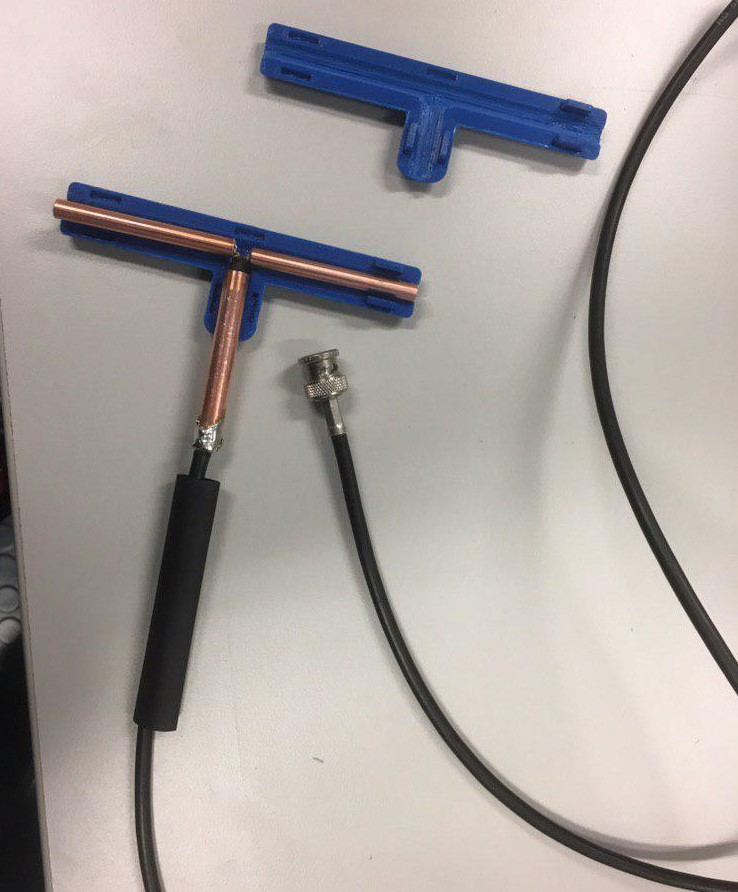
\includegraphics[scale=0.25]{Bilder/Ant_innen_1}
	\centering
	\caption{Aufbau der ersten gebauten Antenne mit Antennengehäuse und Innenleben.}
\end{figure}
Mit den ersten zwei fertigen Antennen wurden erste Probemessungen gemacht um zu sehen ob in dem erwarteten Frequenzbereich ein Intensitätsmaximum zu finden war. Jedoch konnte man im Frequenzband nichts auffallendes erkennen. Auffällig war ein unregelmäßig auftauchender Peak bei einer Frequenz von $2.4\,$GHz. 

\subsection{Tag 2}
Am nächsten Tag wurden weiter versucht, das HackRF zum laufen zu bringen. Leider startete der RaspberryPi nicht mehr, sodass der gestrige Installationsprozess über Nacht erneut durchgeführt wurde. Außerdem wurden die Antennen weiter getestet. Eine mögliche Lösungen für das Problem von ihnen war die Entfernung des Gehäuses, welche aber zu keinen besseren Ergebnissen geführt hat. Auch andere Positionen im Raum führten zum selben Ergebnis, dass kein besonderes Intensitätsmaximum empfangen wurde. Es machte sich jedoch schnell bemerkbar, dass der Raum einem Resonator entspricht und kleine Änderungen im Aufbau des Raum größere Unterschiede bezüglich der Übertragenen Leistung machte. Da kein Messgerät zur Messung der Antennengüte vorhanden war wurde versucht die Frequenz durch auftragen der maximalen empfangenen Leistung. Da diese Nicht aufschlussreich waren, wurde versucht das Stehwellenverhältnis (SWV oder SWR) mittels des Spectrum Anaylzers zu bestimmen. Leider war dies erfolglos, da wir keinen Richtkoppler zu diesem Zeitpunkt zur Verfügung hatten.
\subsection{Tag 3}
Am Mittwoch war das HackRF vollständig einsetzbar, es wurde nun mit einem anderen RasberryPi betrieben. Dies nutzten wir um eine erste Polarisationsmessungen durchzuführen. Auch hier zeigte sich, dass Bewegung von Personen im Raum oder das öffnen eines Fensters die Messwerte stark beeinflusste. Im laufe des Tages erhielten wir einen Richtkoppler, mit welchem die Güte der Antenne gemessen werden konnte. Hier stellte sich heraus die Antennen insgesamt eine sehr Ineffektive Charakteristik hatten und auf keinem Frequenzband relativ effizient sendeten. Da zusätzlich ein Kurzschluss bei einer der Antennen auftrat, wurden zwei neue mit einem Optimierten Design erstellt. Hierbei wurde kein drittes Kupferrohr als Balun senkrecht zum Dipol eingesetzt, sondern die beiden Arme der Antenne wurden direkt mit einer BNC Buchse verbunden.\textcolor{red}{Bild} Beim Test der neuen Antennen zeigt sich eine deutliche Verbesserung zur ersten Generation. Durch des Spectrum Analyzer mit Richtkoppler konnte recht genau gezeugt werden, dass unsere Antennen im erwarteten Bereich besonders gut senden können.\textcolor{red}{Bild} Da beide trotzdem leichte Unterschiede in der Frequenz auftraten, wurde eine mithilfe eines eingebauten Kondensators auf die andere getrimmt.\textcolor{red}{Bild} 
\subsection{Tag 4}
Mit den nun aufeinander genormten Antennen wurde beschlossen, sich auf eine  Polarisationsmessung und Abstandmessung zu beschränken und die Messung der Strahlungscharakteristik wegzulassen. Da jedoch auffällig war wie Problematisch die Umgebung des Labors war, wurden diese Messungen im Labor so wie im Garten der Physik und am Parkplatz vor dem Westbau durchgeführt.
\subsection{Tag 5}
Am letzten Tag wurden noch zusätzliche Messungen zum Abstand und zur Polarisation im Großen Hörsaal durchgeführt. Da die Messungen im Labor bis dahin wegen Bewegung von Personen sehr ungenau war wurde hier nochmal eine Messung durchgeführt, um zu zeigen wie groß die Schwankungen sind und eine bei der sich wirklich nichts verändert. \textcolor{red}{Messung? Unterkapitel mit Bildern und etwas Text da häufig erwähnt}
Anschließend wurden noch weitere Richtkoppler der Werkstatt getestet, ob diese sich wie der geliehene verhalten.
\begin{figure}[h]
	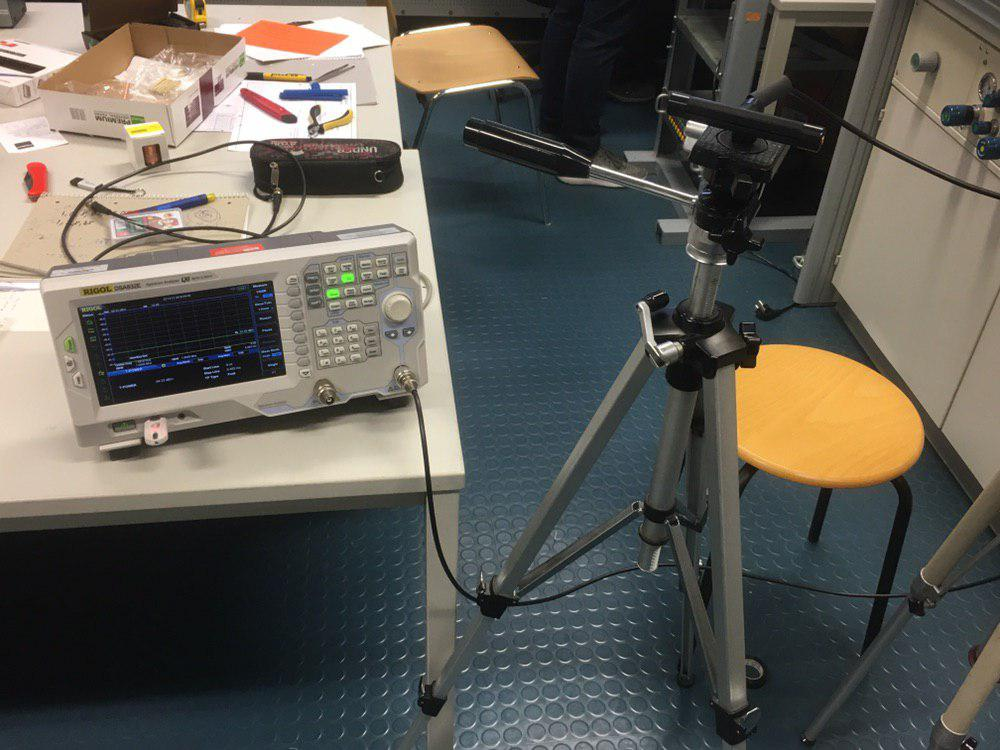
\includegraphics[scale=0.3]{Bilder/Ant_Fktgen}
	\centering
	\caption{Gebaute Antenne auf dem Stativ und an den Frequenzgenerator angeschlossen.}
\end{figure}
\begin{figure}[h]
	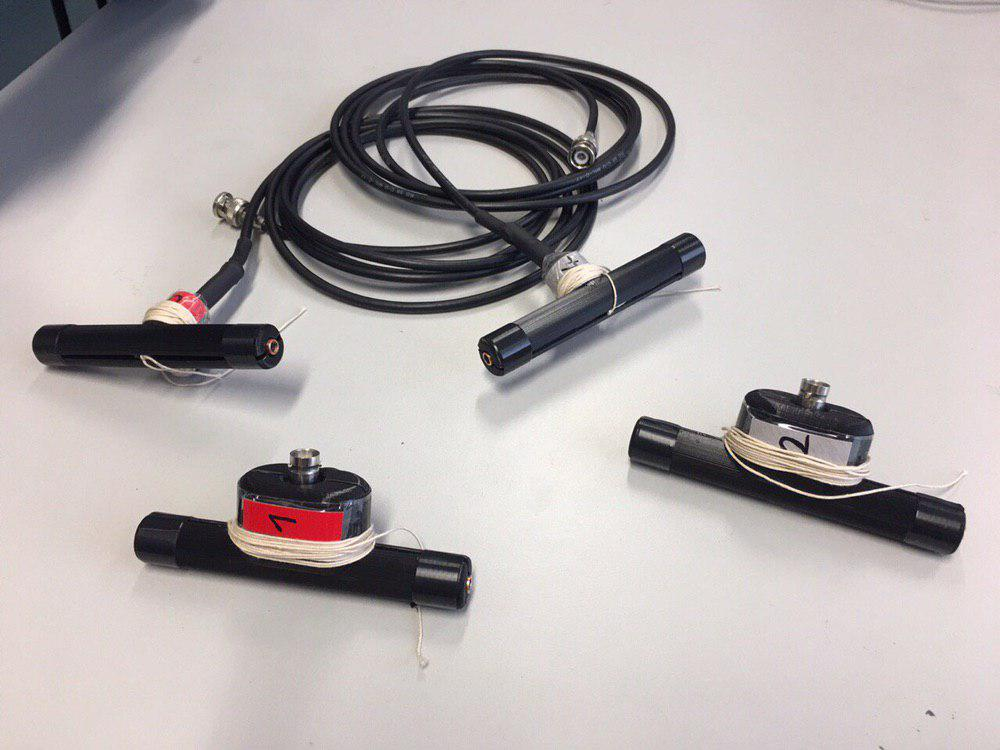
\includegraphics[scale=0.3]{Bilder/Ant_12}
	\centering
	\caption{Beide Antennen Generationen nebeneinander. Hinten die erste Generation vorne die 2.Generation}
\end{figure}
\begin{figure}[h]
	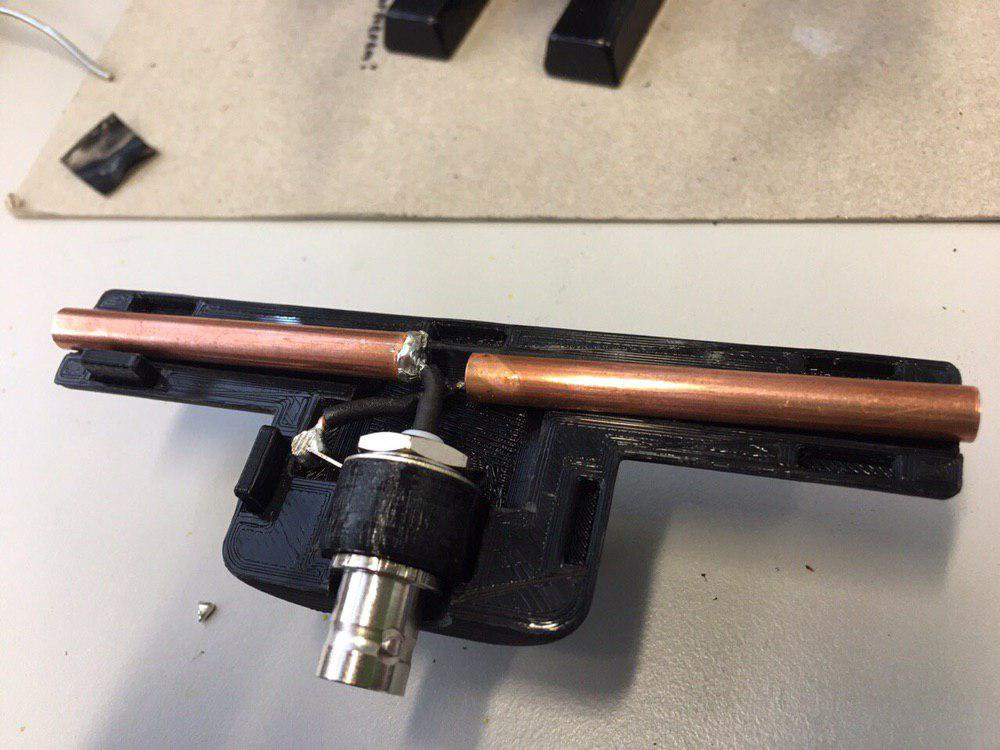
\includegraphics[scale=0.3]{Bilder/Ant_innen_2}
	\centering
	\caption{Innerer Aufbau der 2.Antennengeneration. Im Bild die genormte Antenne mit kleinem Kondensator an der Seite.}
\end{figure}


\section{Details zu den verwendeten Antennen}

\subsection{Antennenbau}
\subsubsection{Erste Generation}
Die erste Antennengeneration wurde nach der Anleitung vom Akademisk Radioklubb gebaut. Diese bestand aus drei $55\,$mm langen Kupferrohren mit einer Wandstärke von $1\,$mm. Hiervon wurden zwei der Rohre, wie bei einem Dipol erwartet, nebeneinander an Kern und Abschirmung eines halbierten Koaxialkabels mit BNC Buchse gelötet. Das dritte Rohr wurde etwas unterhalb der beiden Antennenarme am Kabel als Balun zur Wandlung zwischen dem voraussichtlich asymmetrischen gesendeten Signal und dem symmetrischen Dipolfeld angelötet.

\textcolor{red}{Bild}

\subsubsection{Zweite Generation}

 Diese haben im Gegensatz zu dem alten Modell keinen Balun (bestehend aus einer Kupferröhre um das Signalkabel) mehr.\par
Die Antennen bestehen also nur aus zwei $55\,$mm langen Kupferrohren, die jeweils an Leitung und Schirm eines BNC Gehäuseanschlusses gelötet wurden. Diese Konstruktion wird in einem 3D-gedruckten Gehäuse montiert, sodass die Röhrchen parallel zueinander und orthogonal zum Signalkabel sind. Der nun im Gehäuse eingebaute BNC Anschluss kann nun wie sonst üblich mit kompatiblen Geräten (Oszilloskop, Spectrum Analyzer, etc.) verbunden werden. Dieses Design ist also nicht mehr an ein Kabel gebunden, was den Vorteil hat, dass die Länge variabel ist und ein schlechtes Kabel schnell und leicht ausgetauscht werden kann.\par
Die Plastikgehäuse wurden absichtlich so designet, dass sie ohne Metallteile zusammengebaut werden könnte, da diese die Strahlungscharakteristik beeinträchtigen könnten. Der Kunststoff selbst ist sehr dünn und schien keinen Einfluss auf die Messungen nehmen, dies haben wir rein qualitativ überprüft, indem wir das empfange Signal ohne sowie mit Gehäuse verglichen haben und keinen unterschied feststellen konnten.\par
Außerdem haben die Gehäuse eine Befestigung mit Stativ-Gewinde, sodass sie an Standartmäßigen Fotokamera-Stativen befestigt werden können.
\textcolor{red}{Bild Name}

\subsection{Messung der Antennengüte}
Um die Frequenzen, bei welchen unsere gebauten Antennen relativ gut senden und empfangen können zu bestimmen, wurde die reflektierte Leistung der Antennen für verschiedene Frequenzen bestimmt. Hierzu wurde mithilfe des Spectrum Analyzers ein Frequenzbereich von einigen MHz bis zu $3\,$GHz auf die Antennen gesendet. Dieses Signal wurde dann über einen Richtkoppler auf die zu testende Antenne geleitet, welche dann einen Teil des Signals abstrahlt oder in die Leitung reflektiert. Dieser reflektierte Teil wird über den Richtkoppler zur Messung ausgekoppelt. Beim vermessen der Antennen muss zusätzlich die Charakteristik von Kabeln und dem verwendeten Richtkoppler berücksichtigt werden, worauf wir aber leider nicht genauer eingehen können. Die in diesem Zusammenhang erhobenen Daten befinden sich in der angefügten Messwertesammlung. Zur Bestimmung charakteristischer Frequenzbänder haben wir nur einen Ausgleich mittels des Spectrum Analyzers vorgenommen, welcher die reflektierte Leistung des Richtkopplers und einer $50\,\Omega$  Dummyload normalisierte. Somit erhielten wir für unsere Zwecke brauchbare Charakteristiken. 
\textcolor{red}{Bild Beispielcharakteristik}
\textcolor{red}{Bild Aufbau}

\subsection{Vergleich der Antennen}
Wie im vorherigen Abschnitt besprochen haben wir die Charakteristiken der vier Antennen aufgenommen und verglichen.
\textcolor{red}{Bilder der 4 Messungen "ant 1... ant4" oder so}
Hierbei wurde deutlich, dass die Antennen erster Generation eine komplett andere Charakteristik aufweisen als erwartet, wogegen die Antennen der zweiten Generation sich erwartungsgemäß verhalten. Aufgrund des dipolartigen Aufbaus der Antennen wurde ein relativ breiter Bereich von Resonanz erwartet mit einigen Resonanzen bei Vielfachen der ursprünglichen Resonanzfrequenz. Wie aus den Bildern entnehmbar ist, kann dieses Verhalten nur bei Antennen zweiter Generation beobachtet werden, die vorherigen haben kein klares Minimum an reflektierter Leistung.


\subsection{Trimmen der Empfangsantenne}
Wie in den Bildern zur Reflektionscharakteristik der zweiten Generation Antennen ersichtlich, besitzen beide ein Leistungsminimum in einer Ähnlichen Region. Antenne 2 war das Reflektionsleistungsminimum jedoch deutlich von der Zielfrequenz bei ca. $1.3\,$GHz abgewichen, sodass wir uns entschieden die Impedanz der Antenne auf das richtige Band zu trimmen. Da wir eine relativ feine Anpassung vornehmen wollten, entschieden wir uns variable Kondensatoren parallel zu den Antennenarmen schalten. Wir erhielten drei verschiedene Drehkondensatoren, wobei der mit größter Kapazität am ende verwendet wurde. An diesen wurden zwei Kabel gelötet und an die Antennenarme gedrückt. Nach einigem Herumprobieren entschieden wir uns für eine Position ca. $\frac{2}{3}$ der Stablänge gesehen von den Lötstellen aus. Wir bemerkten, dass die eingestellte Kapazität des Drehkondensators kaum eine Auswirkung auf die Charakteristik hatte, aber die Positionsänderung der Drähte einen großen Einfluss hatte. Vermutlich ist dies durch die Induktivität der Kabel erklärbar. Die induktive Impedanz steigt linear mit der Frequenz, während die kapazitive mit steigender Frequenz fällt. 
\textcolor{red}{Bild der getrimmten Antenne: Aufbau, Vorher nachher chara}

\subsection{Vergleich der Richtkoppler}
Es wurden zusätzlich zum Richtkoppler, mit welchem wir die Messungen zur Antennengüte und das Trimmen durchführten, weitere Richtkoppler bereitgestellt. Als diese nach oben beschriebenen Verfahren zur Messung der nicht getrimmten Antenne der zweiten Generation verwendet wurden, wurde eine völlig unterschiedliche Charakteristik angezeigt. Etwa als würde die Antenne nahezu das gesamte Signal reflektieren. Dies kann aber nach den geglückten Fernfeldmessungen nicht der Fall sein.
\textcolor{red}{Bild Vergleich Richtkoppler}

\section{Versuchsaufbau für die Messungen} 
\subsection{Die Antennen}

Für die ausgewerteten Messungen haben wir nun ausschließlich die neuen Antennen verwendet. Es existieren quantitative Messungen mit den Antennen erster Generation, jedoch fehlte die Zeit auch diese auszuwerten.

\subsection{Der Aufbau zur Vermessung}

Für die jeweiligen Messung haben wir die beiden Antennen an Stativen befestigt und gegenüber voneinander platziert. Die Gehäuse der Antennen wurden an einer dafür vorgesehenen Öse mit einer Schnur verbunden, um die Parallelität der Antennen bei der Anstandsmessung beziehungsweise einen akkuraten Winkel bei der Polarisationsmessung zu gewährleisten.\par
Beide Antennen wurden an den Spectrum Analyzer angeschlossen. Der Spectrum Analyzers schickt nun Signale mit nacheinander gesendeten verschiedenen Frequenzen durch das gesamte Frequenzband des Spectrum Analyzers an die Sender-Antenne und zeichnet die Intensität des von der Empfänger-Antenne kommenden Signals auf.\par
Ein Vorteil an dieser Messung gegenüber dem Senden einer Frequenz über das Hack-RF ist, das wir so auch leicht Störsignale, die von der Antenne empfangen werden feststellen können und damit ausschließen können, dass wie so ein Störsignal mit in die Messung einbeziehen. Hierbei sind Störsignale wie z.B. WLAN oder andere zeitlich nicht konstante Funksignale gemeint. Außerdem können wir dann nicht nur die Peak-Werte auslesen sondern auch 

\subsection{Polarisation}
Zur Messung der Polarisation wurden die Beiden Antennen in einem festen Abstand voneinander auf dem jeweiligen Stativ befestigt. Zum Test ob die Antennen Rechtwinkelig voneinander sind wurde ein Faden genutzt der zwischen beiden Antennen gespannt wurde und dann mit Hilfe eines Geodreiecks ein Rechter Winkel zwischen Antenne und Faden gemessen wurde. Der Sender und Empfänger wurden dann an das Frequenzspektrometur angeschlossen. Zur eigentlichen Messung wurde die Leistungsdifferenz zwischen Sender und Empfänger bei unterschiedlichen Winkeln des Empfängers gemessen.

\section{Auswertung}
Bei der Auswertung unserer Messwerte haben wir uns auf die Abstandsmessungen und die Polarisationsmessungen mit den Antennen zweiter Generation beschränkt. Hierzu werden wir beispielhaft sowohl eine Abstandsmessung als auch eine Polarisationsmessung auswerten. Die restlichen Ergebnisse sind im Anhang zu finden und werden dann im Abschnitt  ,,Diskussion der Ergebnisse`` diese genauer betrachten und interpretieren. \par 
Zuerst betrachten wir die Abstandsmessungen im Großen Hörsaal.Dazu prüfen wir nun ob unsere Messungen sich im Fernfeld oder im Nahfeld der Sendeantenne bewegt. Hier nutzen wir die Näherung:
\begin{equation}
r_{\tx{ff}} \geqslant 2\cdot\lambda
\end{equation}
Damit ist gemeint ab $r_{\tx{ff}}$ beginnt das Fernfeld. Jedoch ist das nur eine Näherung. Tatsächlich ist der genaue Übergang zwischen Fern- und Nahfeld keine eindeutige Grenze sondern dazwischen liegt der Übergangsbereich, welcher die Abgrenzung zwischen Nahfeld und Fernfeld erschwert. Jedoch soll für unsere Abstandmessung diese Näherung ausreichend sein, da, wie man gleich sehen wird, wir uns bei dem meisten Messwerten mit Sicherheit im Fernfeld bewegen. \par 
Um nun $r_{\tx{ff}}$ für unsere Sendeantenne zu berechnen, berechnen wir zunächst die Wellenlänge $\lambda$ für unsere Sendefrequenz $f=1{,}616\,$GHz mit einem Ablesefehler von $\Delta f=0{,}0005\,$GHz ($c\approx 3\cdot10^{8}\,\frac{\tx{m}}{\tx{s}}$). Damit erhalten wir für die Wellenlänge und den Fehler (mittels Gauß'scher Fehlerfortpflanzung) folgende Werte:
\begin{equation*}
\lambda = \frac{c}{f} \approx 0{,}1856\,\tx{m} \qquad \qquad
\Delta \lambda = \frac{\Delta f c}{f^{2}} \approx 1{,}1 \cdot 10^{-4}\,\tx{m}
\end{equation*}
Somit erhalten wir für das Fernfeld einen Mindestabstand von: 
\begin{equation*}
r_{ff} \geqslant 2\cdot\lambda = 0{,}3713\,\tx{m}\, \pm 2\cdot10^{-4}\,\tx{m}
\end{equation*}
Somit können wir sagen wir bewegen uns bei unseren Abstandsmessungen im Fernfeld, da bei allen Messungen höchstens ein bis zwei Werte unter $r_{\tx{ff}}$ liegen (siehe Messwerte im Anhang). \par 
Als nächstes berechnen wir die Leistung der Messwerte in W, da sie noch in dBm angegeben sind. Dazu nutzen wir die Formel:
\begin{equation}
\tx{I in Watt}: 10^{\frac{(I[dBm]-30)}{10}}
\end{equation}
Die Fehler haben wir auf Grund der Schwankungen des Messpunktes auf $\Delta I=$$\pm 1\,$dBm geschätzt. Damit ist dieser Fehler deutlich größer als die aus den Impedanzen des Spectrum Analyzers (aus den Herstellerinfos), so das wir diese vernachlässigen können. Da diese Fehler auf Grund der logarithmischen Messwerte asymmetrisch sind, und wir aber gleich große Fehler in beider Richtungen haben wollen, rechnen wir:


\bibliographystyle{plain}
\bibliography{literature}
\addcontentsline{toc}{section}{Literatur}
%\bibitem[Antennenbauanleitung]{https://www.la1k.no/2017/10/25/a-quick-sleeve-metal-dipole-for-23-cm/}
%Hallo23
\end{document}
